% !TeX root = ../../../master.tex

\subsection{Teilnahme Umfrage}
\label{ssec:UmfrageImplement}

Wie in \abb \vref{fig:UmfrageImplement} dargestellt, soll der Teilnehmer hier auf den zuvor erstellten Frageboge geleitet werden (vgl. Kap. \vref{ssec:UmfrageErstellen}). 
Hier kann dieser diesen ausfüllen und nach Beendigung über einen Button abschicken. 
% Der Teilnehmer erhält am Ende ein visuelles Feedback, dass seine Teilnahme erfolgreich war.

\abb \vref{fig:UmfrageImplement} stellt eine Umfrage zur Projektmanagement-Vorlesung dar, in der der Teilnehmer drei Fragen beantworten soll. 
Exemplarisch sind hier bei drei Fragetypen angeführt: 
\begin{itemize}
	\item Multiple Choice: Auswahl der Notationsart für zukünftige Projekte
	\item Skala: Benotung der Vorlesung auf einer Skala von 1 - 5
	\item Ja/Nein: Ob der Teilnehmer die Vorlesung erneut besuchen würde 
\end{itemize}

Über den Button \jinline|Complete| kann der Teilnehmer die Umfrage beenden. 
Er erhält ein visuelles Feedback über seine Teilnahme.

\begin{figure}[hp]
	\centering
	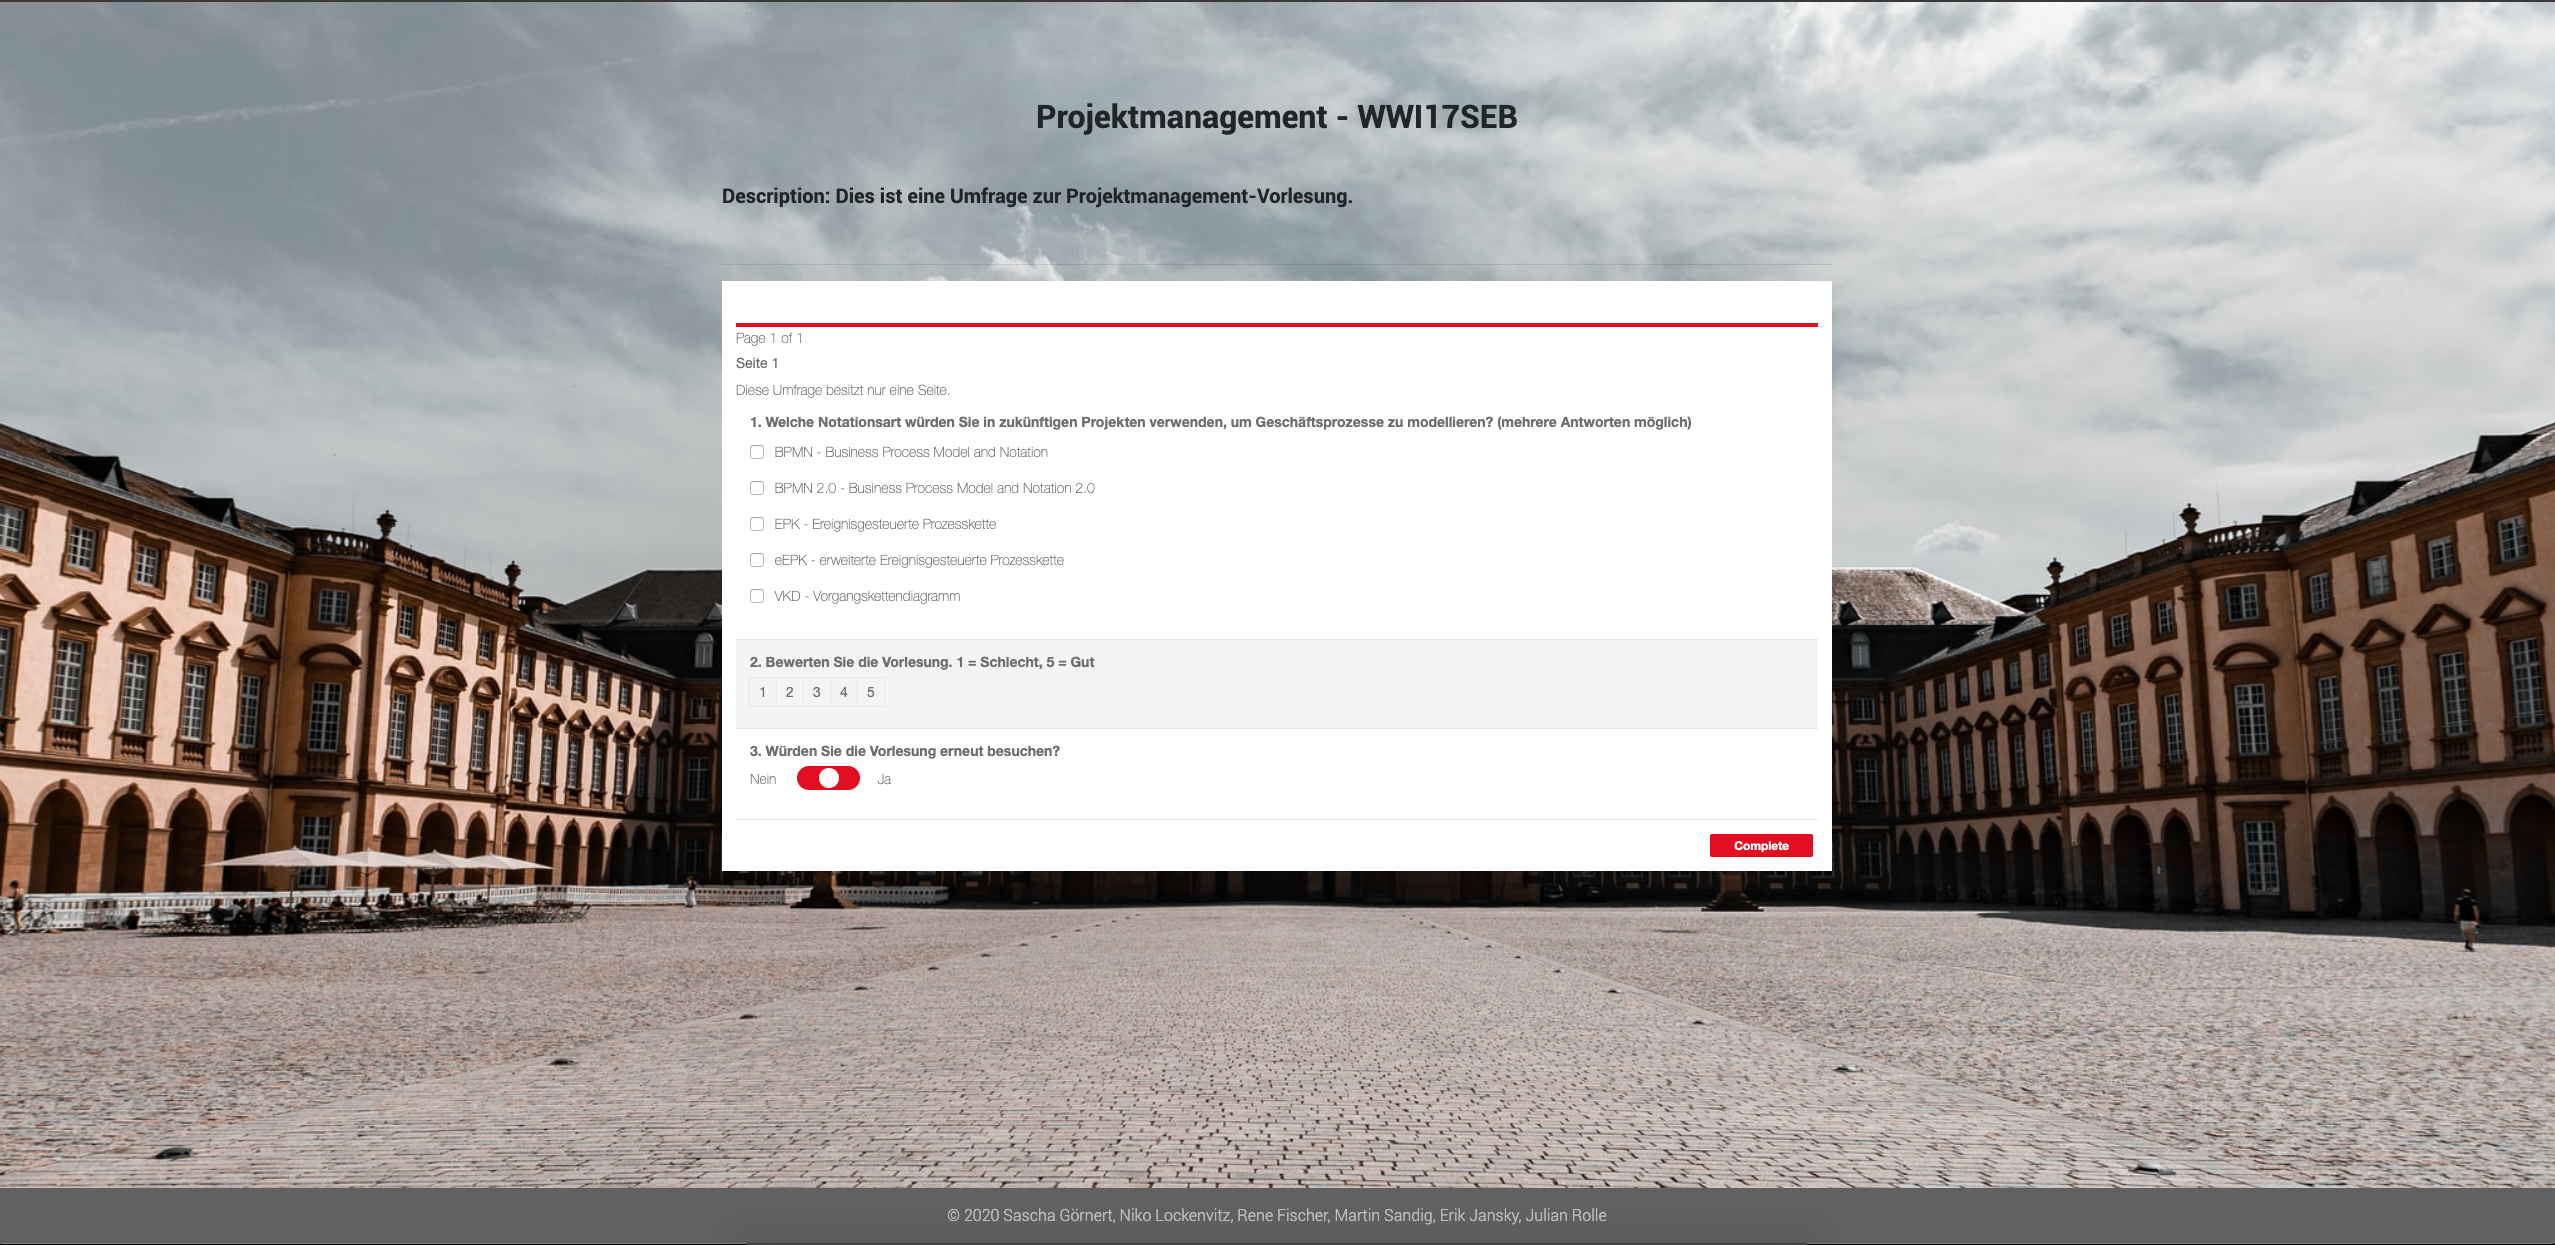
\includegraphics[width=0.95\textwidth, keepaspectratio]{img/client/TeilnahmeUmfrage.png}
	\captionsetup{justification=centering, format=plain}
	\caption[\acf{UI}: Umfrageansicht -- Teilnehmer]{\acf{UI}: Umfrageansicht -- Teilnehmer \\ \quelleScreenshot}
	\label{fig:UmfrageImplement}
\end{figure}
